\cotefile{34}
\scanpage{18}
\mspage{16}
% archive sheet number: 17
% hand: Grothendieck
% sheet_kind: text
% element: text | top, line 1 | 4. Généralités
\deleted{\unsure{3}}4. \uline{Généralités sur les représentations $\ell$-adiques de $I$} $(\ell\ne p)$.

% element: text | upper, line 2 | Soit E un module
Soit $E$ un module de type fini sur $\mathbb Z_\ell$, donc
% element: display | upper, line 3 | E = lim E_nu
\[
E=\varprojlim_\nu \underbrace{E_\nu\deleted{\unsure{\otimes\mathbb Z/\ell^{\nu+1}\mathbb Z}}}_{E_\nu},\qquad E_\nu=E\otimes_{\mathbb Z_\ell}\mathbb Z/\ell^{\nu+1}\mathbb Z.
\tag*{(4.1)}
\]
% element: text | upper, line 4 | d'où
d'où
% element: display | upper, line 5 | G = Aut(E)
\[
G=\operatorname{Aut}_{\mathbb Z_\ell}(E)=\varprojlim_\nu\operatorname{Aut}_{\mathbb Z/\ell^\nu\mathbb Z}(E_\nu)
\tag*{(4.2)}
\]
% element: text | upper-middle, lines 6–8 | Par définition
Par définition, on munit $\operatorname{Aut}_{\mathbb Z_\ell}(E)$ de la structure de groupe topologique profini, limite projective des groupes finis apparaissant dans (4.1). Notons le

% element: text | middle, line 9 | Lemme 4.3
\uline{Lemme} 4.3 Le \deleted{\unsure{groupe}}\unsure{ss.-groupe} \deleted{\unsure{de}}
% element: display | middle, line 10 | G^1 = Ker
\[
G^1=\operatorname{Ker}\bigl(\operatorname{Aut}_{\mathbb Z_\ell}(E)\longrightarrow\operatorname{Aut}_{\mathbb Z/\ell\mathbb Z}(E_0)\bigr)
\]
% element: text | middle, lines 11–12 | est un sous-groupe
est un \unsure{sous-groupe|ss-groupe} ouvert de $G$, \deleted{\unsure{qui}} et c'est un pro-$\ell$-groupe.

% element: text | lower-middle, lines 13–15 | Dém.
\uline{Dém.} Le fait qu'il soit ouvert est trivial par définition. Que ce soit un pro-$\ell$-groupe \deleted{\unsure{est}} provient du fait que pour $\nu\geq 1$,
% element: display | lower-middle, line 16 | Ker(Aut(E_nu) to Aut(E_0))
\[
\operatorname{Ker}\bigl(\operatorname{Aut}(E_\nu)\longrightarrow\operatorname{Aut}(E_0)\bigr)
\]
% element: text | lower, lines 17–24 | est un l-groupe
est un $\ell$-groupe. Or si $u$ est tel que $u\equiv\operatorname{id}\;(\ell)$ \deleted{\unsure{i.e.} $(u-\unsure{1})(E_\nu)\subset\ell E_\nu$, on conclut par récurrence \unsure{que} $(u-1)^{\unsure{i}}\subset\ell^iE_\nu$, d'où pour $i=\nu+1$, $(u-1)^{\unsure{\nu}}E_\nu=0$, ce qui} alors $u$ induit l'identité sur le gradué associé à $E_\nu$ par la filtration (finie) \inserted{$\ell$-adique} (par les $\ell^iE_\nu$), d'où on conclut facilement par récurrence \inserted{sur $r$} que $u^{\ell^r}$ induit l'identité sur le

\scanpage{19}
\mspage{17}
% archive sheet number: 18
% hand: Grothendieck
% sheet_kind: text
% element: text | top, lines 1–2 | gradué associé
gradué associé à la filtration $\ell^r$-adique (par les $\ell^{ri}E_\nu$). Faisant $r=\nu+1$, on gagne.

% element: text | upper, lines 3–6 | Corollaire 4.4
\uline{Corollaire} 4.4. Pour tout \deleted{sous-groupe} fermé $Q$ de $G$ qui est une \deleted{pro-$p$ groupe $(p\ne\ell)$}\inserted{limite projective de} groupes finis d'ordre premiers à $\ell$, \deleted{l'image} l'hom. naturel
% element: display | upper, line 7 | Q to Aut(E_0)
\[
Q\longrightarrow\operatorname{Aut}_{\mathbb Z/\ell\mathbb Z}(E_0)
\]
% element: text | upper, line 8 | est injectif
est injectif; en particulier $Q$ est fini.

% element: text | middle, lines 9–13 | Corollaire 4.5
\uline{Corollaire} 4.5. Soit $u:I\longrightarrow G$ un \deleted{\unsure{épimorphisme}}\inserted{hom continu} \unsure{arbitraire} \unsure{$\ell$|6} (où $I$ comme au n° 2), \inserted{et $N=\operatorname{Ker}u$.} \deleted{Alors} Soit $I'$ \deleted{\unsure{le}} l'image inverse dans $I$ du sous-groupe $\prod_{\ell'\ne\ell,p}\mathbb Z_{\ell'}(1)$ de $I/\unsure{p|P}\simeq\prod_{\ell'}\mathbb Z_{\ell'}(1)$, \deleted{Alors} Alors l'hom induit
% element: display | middle, line 14 | I'/I' cap N to Aut(E_0)
\[
I'/I'\cap N\longrightarrow\operatorname{Aut}_{\mathbb Z/\ell\mathbb Z}(E_0)
\]
% element: text | lower-middle, lines 15–16 | est injectif
est injectif, en particulier $I'/I'\cap N$ est un groupe fini, i.e. $I'\cap N$ est ouvert dans $I'$.

% element: text | lower, lines 17–20 | Par suite
Par suite, il existe un \deleted{certain} sous-groupe ouvert $U$ dans $I$ tel que $U\cap I'\subset I'\cap N$, p.ex. \deleted{\unsure{dans le}} $U=\operatorname{Ker}(G\longrightarrow\operatorname{Aut}_{\mathbb Z/\ell\mathbb Z}(E_0))$. Alors l'hom induit
% element: display | lower, line 21 | U to G
\[
U_{\deleted{\unsure{\ell}}}\longrightarrow G
\]
% element: text | bottom, lines 22–23 | s'annule sur U cap I'
s'annule sur $U\cap I'$, donc passe au quotient en un hom
% element: display | bottom, line 24 | U/U cap I' = Im
\[
U/U\cap I'=\operatorname{Im}(U\longrightarrow\mathbb Z_\ell(1))\longrightarrow G\deleted{\unsure{\operatorname{Aut}_{\mathbb Z_\ell}(E)}}.
\]

\scanpage{20}
\mspage{18}
% archive sheet number: 19
% hand: Grothendieck
% sheet_kind: text
% element: text | top, line 1 | En d'autres termes
En d'autres termes:

% element: text | upper, lines 2–5 | Corollaire 4.5
\uline{Corollaire} 4.5. Avec les notations de \unsure{4.4}, quitte à \deleted{\unsure{par}} la restreindre à un sous-groupe ouvert \inserted{convenable} $U$ de \unsure{$\pi$|$I$}, la représentation donnée $u:I\longrightarrow G$ se factorise en une représentation
% element: display | upper, line 6 | U to Im(U to Z_l(1)) to G
\[
U\longrightarrow\operatorname{Im}(U\longrightarrow\mathbb Z_\ell(1))\unsure{-|\longrightarrow}G
\]
% element: text | upper-middle, lines 7–8 | d'un sous-groupe ouvert
d'un sous-groupe ouvert \inserted{$U'$\deleted{\unsure{$U$}}} du facteur \deleted{\unsure{$\mathbb Z_\ell(1)$}} $\ell$-primaire $\mathbb Z_\ell(1)$ de $I_t$.

% element: text | middle, lines 9–10 | Si l^nu est l'indice
Si $\ell^\nu$ est l'indice de ce dernier, alors la multiplication par $\ell^\nu$ induit un isomorphisme
% element: display | middle, line 11 | Z_l(1) isom U'
\[
\mathbb Z_\ell(1)\xrightarrow{\sim}U',
\tag*{(4.7)}
\]
% element: text | middle, lines 12–14 | et on est donc ramené
et on est donc ramené, pour étudier la restriction de $u$ à $U$, à étudier une représentation $\ell$-adique du groupe $\mathbb Z_\ell(1)$.

% element: text | lower-middle, lines 15–16 | En fait, souvent
En fait, souvent on se borne à prendre $U$ tel que
% element: display | lower-middle, lines 16–17 | P cap U subset P cap N
\[
\begin{aligned}
&\deleted{\unsure{K\subset N}\quad K\cap U\subset\unsure{K}}\\
&P\cap U\subset P\cap N,
\end{aligned}
\]
% element: text | lower, lines 18–19 | de sorte que la restriction
de sorte que la restriction de $u$ à $U$ se factorise en un hom
% element: display | lower, line 20 | U' = Im(U to I_t) to G
\[
U'=\operatorname{Im}(U\longrightarrow I_t)\longrightarrow G.
\]
% element: text | lower, line 21 | Ici encore
Ici encore, on trouve un isom canonique
% element: display | lower, line 22 | U' isom I_t isom product
\[
U'\simeq I_t\simeq\prod_{\ell'\ne p}\mathbb Z_{\ell'}(1)
\tag*{(4.8)}
\]
% element: text | bottom, line 23 | On retiendra
On retiendra en particulier que $U'$ est \uline{commutatif}.

% element: text | bottom edge, lines 24–27 | 4.9 On peut aussi exprimer
\inserted{4.9.} On peut aussi exprimer ceci en disant que, quitte à faire une extension séparable finie $K_1$ de $K$, la repr. $\ell$-adique donnée de $I$ définit une repr. $\ell$-adique \unsure{de $I_1$} qui se factorise par sa ``partie $\ell$-primaire'' $\unsure{I(\ell)|I_1(\ell)}=\mathbb Z_\ell(1)$.

\scanpage{21}
\mspage{19}
% archive sheet number: 20
% hand: Grothendieck
% sheet_kind: text
% element: text | top, lines 1–3 | 4.10 Parfois
4.10. Parfois on aura à considérer un vectoriel de dim finie $E$ sur $\mathbb Q_\ell$, et une représentation continue
% element: display | upper, line 4 | u: pi to Aut(E)
\[
u:\pi\longrightarrow\operatorname{Aut}_{\mathbb Q_\ell}(E)
\tag*{(4.10.1)}
\]
% element: text | upper, lines 5–8 | Le fait à retenir
Le fait à retenir est que ($\pi$ étant compact) il existe toujours un ``réseau invariant'' par $\pi$, i.e. un sous-$\mathbb Z_\ell$-module $E_{\mathbb Z_\ell}$, \deleted{tel que} libre de type fini sur $\mathbb Z_\ell$, stable par $\pi$, tel que
% element: display | upper-middle, line 9 | E_Z_l tensor Q_l isom E
\[
E_{\mathbb Z_\ell}\otimes_{\mathbb Z_\ell}\mathbb Q_\ell\xrightarrow{\sim}E,
\]
% element: text | middle, insertion before line 10 | donc u se factorise
\deleted{\unsure{donc}}\inserted{donc $u$ se factorise \inserted{(4.10.1)}}
% element: display | middle, line 10 | u_Z_l: pi to Aut_Z_l
\[
u_{\mathbb Z_\ell}:\pi\xrightarrow{\sim}\operatorname{Aut}_{\mathbb Z_\ell}(E_{\mathbb Z_\ell})
\tag*{(4.10.2)}
\]
% element: text | middle, lines 11–15 | Il s'ensuit
Il s'ensuit \inserted{donc} que pour \unsure{tt|tout|$\forall$} sous-groupe $Q$ de $\pi$ qui est $\simeq$ une limite projective de groupes finis d'ordre \unsure{premier|premiers} à $\ell$, $u(Q)$ est un sous-groupe fini de $G=\operatorname{Aut}_{\mathbb Q_\ell}(E)$, et les cor. 4.5, et 4.6\ldots\ sont applicables.

% element: text | lower-middle, line 16 | 5. Représentations quasi-unipotentes
5. \uline{Représentations quasi-unipotentes}.

% element: text | lower, lines 17–24 | Définition 5.1
\uline{Définition} 5.1 Soit $\pi$ un groupe profini; $u:\pi\longrightarrow\operatorname{Aut}_R(E)$ une représentation linéaire de $\pi$, \deleted{\unsure{par}} \unsure{autom.} d'un vectoriel de dim finie sur \inserted{un corps} $R$. On dit que $u$ est \deleted{\unsure{quasi}} \uline{unipotente} si $\forall g\in\pi$, $u(g)$ est un automorphisme unipotent de $E$, i.e. ses valeurs propres (dans une cloture alg. de $R$) sont toutes égales à $1$, ou encore son polynôme car. $\det(\deleted{\unsure{\pi}}T\operatorname{id}-u)$ est égal à $T^n-1$. On dit que

\scanpage{22}
\mspage{20}
% archive sheet number: 21
% hand: Grothendieck
% sheet_kind: text
% element: text | top, lines 1–3 | la représentation
la représentation \inserted{$u$} est \uline{quasi-unipotente} s'il existe un sous-groupe ouvert $U$ de $\pi$ tel que la représentation induite $u\mid U$ soit unipotente.

% element: text | upper-middle, lines 4–13 | 5.2 Supposons R infini
5.2. Supposons $R$ infini, et soit $G$ le groupe algébrique engendré par $u(\pi)$, \deleted{Alors} c.à.d. l'adhérence (avec structure induite réduite) de l'ens $u(G)$ dans le schéma en groupes des autom. de $E$. Comme l'ensemble des \deleted{\unsure{pts} de}\inserted{automorphismes} \deleted{\unsure{Aut}} unipotents \deleted{\unsure{constitue}}\inserted{est} une partie Zariski-fermée de l'ens $\operatorname{Aut}(E)$, il s'ensuit que $u$ est unipotent ssi $G$ est unipotent, (i.e. chacun de ses éléments \inserted{sur $\overline R$} est un automorphisme unipotent de $E_{\overline R}$).
% element: margin note | left margin, beside lines 11–14 | Noter que G/G^0
\margin{Noter que $G/G^\circ$ est un groupe \deleted{\unsure{et}} quotient isom. à $\pi/U$, où $U$ est l'image inverse de $G^\circ(R)$}

% element: text | middle-lower, lines 13–19 | 5.3 Si R est un corps
\deleted{\unsure{Dém.|De même}}\inserted{5.3.} Si $R$ est un corps topologique \inserted{séparé}, et $u$ est continue, alors dire que $u$ est quasi-unipotent revient à dire que $G^\circ$ est unipotent. C'est évidemment suffisant, car l'homomorphisme $\pi\longrightarrow(G/G^\circ)(R)$ \inserted{\unsure{ou} $G(R)/G^\circ(R)$} est continu \inserted{pour la top. discrète sur $G/G^\circ$}, donc l'image inverse de $G^\circ(R)$ est un sous-groupe ouvert \deleted{\unsure{de}} $U$ de $\pi$.
% element: drawing | lower left margin, beside lines 18–20 | tall loops, R and uncertain labels
% crop-candidate: scan 22
\figure{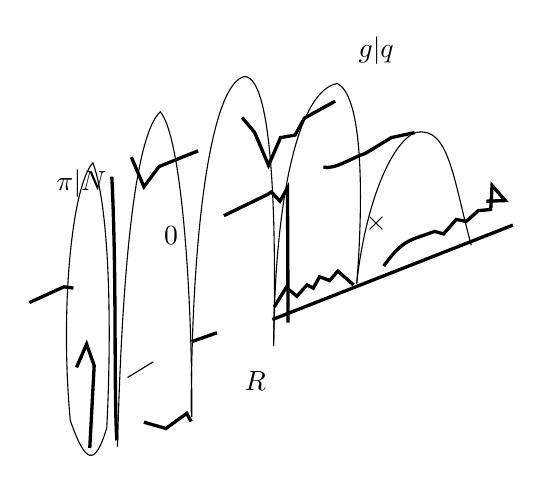
\begin{tikzpicture}[x=0.008cm,y=-0.008cm]
\draw[thin] (65,650)..controls(48,465)and(69,275)..(101,241)..controls(128,315)and(131,505)..(123,662)..controls(104,725)and(89,719)..(65,650);
\draw[thin] (140,692)..controls(147,419)and(167,197)..(208,160)..controls(243,200)and(259,464)..(258,645);
\draw[thin] (257,638)..controls(258,326)and(292,113)..(342,104)..controls(390,105)and(392,370)..(388,530);
\draw[thin] (388,532)..controls(390,288)and(429,126)..(489,115)..controls(537,138)and(527,350)..(520,433);
\draw[thin] (520,432)..controls(535,298)and(578,205)..(614,193)..controls(667,181)and(674,271)..(702,372);
\draw[very thick] (0,463)--(55,438)--(70,440);
\draw[very thick] (386,490)--(768,340);
\draw[very thick] (75,566)--(91,529)--(103,563)--(96,694);
\draw[very thick] (131,263)..controls(139,420)and(134,600)..(139,682);
\draw[very thick] (162,232)--(182,279)--(206,247)--(268,222);
\draw[very thick] (182,653)--(217,663)--(250,639)--(257,652);
\draw[very thick] (258,525)--(298,511);
\draw[very thick] (338,169)--(358,193)--(380,245)--(399,201)--(422,197)--(437,170)--(486,143);
\draw[very thick] (309,325)--(379,291)--(386,286);
\draw[very thick] (385,288)--(398,302)--(410,281)--(411,495);
\draw[very thick] (467,248)..controls(486,252)and(514,232)..(534,226)--(575,201)--(612,193);
\draw[very thick] (389,470)--(408,439)--(425,453)--(441,435)--(451,440)--(461,422)--(477,428)--(490,413)--(515,435);
\draw[very thick] (563,405)..controls(590,366)and(607,363)..(624,357)--(644,350)--(658,354)--(678,331)--(694,334)--(713,317)--(735,315);
\draw[very thick] (733,313)--(735,277)--(756,301)--(726,302);
\draw[thin] (156,582)--(197,557);
\node at(83,274){$\unsure{\pi|N}$};
\node at(359,588){$R$};
\node at(551,63){$\unsure{g|q}$};
\node at(225,356){$\unsure{0}$};
\node at(551,338){$\unsure{\times}$};
\end{tikzpicture}}
% element: text | bottom, lines 19–24 | Inversement
Inversement, si $U$ est un s-groupe ouvert de $\pi$ qui opère de façon unipotente, prenant $U$ assez petit on peut supposer que $U\subset u^{-1}(G^\circ(R))$. Alors $\overline{u(U)}$ est un sous-groupe algébrique \inserted{lisse $H$} de $G^\circ$, donc

\scanpage{23}
\mspage{21}
% archive sheet number: 22
% hand: Grothendieck
% sheet_kind: cancelled_draft
% element: text | top, lines 1–4 | on constate immédiatement
on constate immédiatement qu'\deleted{\unsure{il}} il \unsure{se trouve} $H(\overline R)$ d'indice fini dans $G^\circ(\overline R)$, ce qui implique que $H=G^\circ$; \deleted{donc} comme $H$ est unipotent, il en est de même de $G^\circ$.
% element: margin note | upper left, slanted | dégager un lemme
% slanted
\margin{\unsure{dégager} un lemme, avec le corollaire $E^U=E^{G^\circ}$.}

% element: text | upper-middle, lines 5–7 | 5.4 Supposons maintenant
5.4. Supposons maintenant que $\pi$ opère de façon quasi-unipotente, (\deleted{donc}\inserted{i.e.} $G$ est unipotent) et \uline{supposons que $R$ soit de car. nulle}.

% element: text | cancelled block, lines 7–16 | Si U est un sous-groupe
\deleted{Si $U$ est un sous-groupe \deleted{\unsure{ouvert}}\inserted{invariant} de $\pi$ qui opère de façon unipotente (p.ex $u^{-1}(G^\circ(R))$), on peut former \deleted{\unsure{$F$}} $E^U$, sur lequel $\pi/U$ opère. Je dis que $E^U$ ne dépend pas du choix de $U$; en effet, il suffit de voir que $E^U=E^{U'}$ si $U'\subset U$, $U'$ \uline{invariant}. Or $\pi/U'$ opère sur $E^{U'}$, donc $U/U'$ y opère; c'est un groupe fini qui opère de façon unipotente, donc (puisqu'on est en car nulle) il opère \unsure{trivialt|trivialmt}. De plus, $E^U$ \deleted{\unsure{soit}} \inserted{inv. dans $\pi$ (car on peut supposer $U$ invariant dans $\pi$).}}
% element: text | cancelled line, below line 16 | Ceci nous montre
\deleted{\deleted{Ceci nous montre en particulier que}}
% element: display | cancelled block, line 17 | E^U = E^G^0
\[
\deleted{E^U=E^{G^\circ}.}
\]
% element: text | cancelled block, lines 17–18 | Nous pouvons définir
\deleted{Nous pouvons définir une filtration croissante de $E$, en posant}
% element: display | cancelled block, lines 19–20 | E^(0) = 0
\[
\begin{aligned}
&\deleted{E_{\unsure{0|a}}^{(0)}=0,\qquad E^{(i+1)}=\text{image inverse de}}\\
&\deleted{\deleted{\unsure{(E/E^i)^U=(E/E^i)^{G^\circ}}}}\\
&\deleted{\inserted{(E/E^i)^U=(E/E^i)^{G^\circ}\quad\text{dans }E}.}
\end{aligned}
\]
% element: text | cancelled bottom block, lines 21–24 | L'hypothèse
\deleted{L'hypothèse que \deleted{\unsure{$U$ opère}} $G^\circ$ opère de façon unipotente implique que cette filtration est exhaustive. \deleted{\illegible{1}} D'autre part, $U$ opère \deleted{\unsure{de façon unipotente}}\inserted{trivialmt} sur le gradué associé, par construction. On}

\scanpage{24}
\mspage{22}
% archive sheet number: 23
% hand: Grothendieck
% sheet_kind: cancelled_draft
% element: text | upper, lines 1–7 | Alors je dis que
Alors je dis que \deleted{\unsure{$E$}} \uline{si} $g\in G(R)$, \uline{$g$ est unipotent} ssi $g\in G^\circ(R)$. En effet, \deleted{\unsure{on est réduit|on est déjà}} à prouver \deleted{seulement ``seulement si''. \unsure{Sup}} seulement: $g$ unipotent $\Rightarrow g\in G^\circ(R)$. Or \deleted{\unsure{considérons son}} l'image de $g$ dans le groupe quotient $\Gamma=G/G^\circ$ est un \unsure{élém|élément} \uline{unipotent} de $\Gamma(R)$, et comme on est en car. $0$, c'est l'unité.

% element: text | cancelled middle, lines 7–9 | Pour toute
\deleted{\unsure{Pour toute}\illegible{2} Pour tout dire: on filtre $E$ par $E^0=0,\ldots E^i\ldots,\}$, \unsure{avec} \deleted{$E^i=$\unsure{image inverse de}}}
% element: display | cancelled middle, line 10 | E^(i+1) image inverse
\[
\deleted{E^{i+1}=\text{image inv. dans }E\text{ de }(E/E^i)^{G^\circ}.}
\tag*{(5.4.1)}
\]
% element: text | cancelled middle, lines 11–18 | Cette filtration
\deleted{Cette filtration est \deleted{\unsure{finie}}\inserted{exhaustive, i.e. $\exists i$ t.q. $E^i=E$,} ce qui exprime simplement que $G^\circ$ est unipotent. Alors $G/G^\circ$ opère sur les $E^{i+1}/E^i$, et si $g\in G$ est unipotent, il induit des op. unipotentes dans les $E^{i+1}/E^i$, donc des opérations triviales, i.e. il appartient au \uline{noyau} de $G/G^\circ$ opérant sur $\operatorname{Gr}(E)$. Mais comme on est en car. zéro, \deleted{\unsure{cela implique que}} l'op. de $G/G^\circ$ est \unsure{semi-simple}, donc $E\unsure{\sim|\simeq}\operatorname{Gr}(E)$ \unsure{par un}}

% element: text | lower, lines 19–22 | En particulier
En particulier, l'image inverse $U$ de $G^\circ(R)$ dans $\pi$ est le plus grand ss-groupe de $\pi$ opérant de façon unipotente, et à fortiori le plus grand ss-groupe ouvert ayant cette propriété.

% element: text | bottom, lines 23–27 | 5.5.a Notons
\unsure{5.5.a} Notons que \deleted{\unsure{l'on sait de}}\inserted{la structure} connue des \unsure{groupes alg.} \inserted{unipotents} commutatifs (sur un corps $R$ de car. $0$), comme groupes vectoriels, permet de \deleted{\unsure{faire}} trouver une filtration ``caractéristique'' de $G^\circ$ (par les \inserted{groupes de} commutateurs successifs, $G^{(0)}=G$,

\scanpage{25}
\mspage{23}
% archive sheet number: 24
% hand: Grothendieck
% sheet_kind: text
% element: text | top, lines 1–2 | G^(i+1) = [G^(i),G]
$G^{(i+1)}=[G^{(i)},G]$) tel que $\operatorname{Gr}(G^\circ)$ soit un groupe vectoriel. On en conclut, comme
% element: display | upper, line 3 | H^i(Gamma,V)=0
\[
H^{\unsure{i|\nu}}(\Gamma,V)=0\qquad\text{pour }i\geq0
\]
% element: text | upper, lines 4–7 | et tout vectoriel V
et $\unsure{\text{tt}|\forall}$ vectoriel $V$ sur lequel $\Gamma$ opère (car $V$ est uniquement divisible\ldots), que \uline{l'extension} $G$ de $\Gamma$ par $G^\circ$ \uline{splitte de façon unique en un} produit semi-direct
% element: display | upper-middle, line 8 | G isom Gamma.G^0
\[
G\simeq\Gamma.G^\circ.
\tag*{(5.5.1)}
\]
% element: text | middle, lines 9–11 | Ceci montre que
Ceci \deleted{\unsure{permet de voir que}}\inserted{montre que $\Gamma$ opère de façon naturelle} sur $E$, \deleted{[et permet de retrouver le fait que $\forall g\in G(R)$, \unsure{i.e.} $g$ unipotent $\Rightarrow g\in G^\circ(R)$]}
% element: margin note | left, below cancelled paragraph | (5.6), 5.6
\margin{\deleted{(5.6)}\quad\deleted{5.6}}
% element: text | middle, unfinished last line | Pour t.
\unsure{Pour t.}

\scanpage{26}
\mspage{24}
% archive sheet number: 25
% hand: Grothendieck
% sheet_kind: cancelled_draft
% element: text | cancelled upper block, lines 1–7 | 5.5 On en conclut
\deleted{5.5. On en conclut que \deleted{\unsure{il existe le groupe}}\inserted{l'ens \inserted{$U$}} des $g\in\pi$ tels que $u(g)$ soit unipotent est un sous-groupe ouvert invariant de $\pi$, à savoir $u^{-1}(G^\circ(R))$; c'est évidemment le plus grand sous-groupe \deleted{ouvert} (ou le plus grand sous-groupe ouvert) de $\pi$ \deleted{qui \unsure{y}} opère de façon unipotente. Rappelons que}
% element: display | cancelled upper block, line 8 | pi/U isom (G/G^0)(R)
\[
\deleted{\pi/U\simeq(G/G^\circ)(R)\simeq G(R)/G^\circ(R).}
\tag*{(5.5.1)}
\]
% element: text | cancelled middle, lines 9–11 | Soit U' un sous-groupe
\deleted{Soit $U'$ un sous-groupe \deleted{\unsure{d'indice|fini}}\inserted{(ouvert)} de $\pi$ \deleted{qui opère} de façon unipotente, i.e. un ss-groupe ouvert de $U$, je dis qu'on a alors}
% element: display | cancelled middle, line 12 | E^U' = E^U = E^G^0
\[
\deleted{E^{U'}=E^U=E^{G^\circ}.}
\]
% element: text | cancelled middle-lower, lines 13–17 | En effet
\deleted{En effet, on peut supposer que $U'$ est invariant; alors $U/U'$ opère sur $E^{U'}$, et \deleted{\unsure{et qui}}\inserted{c'est} un groupe fini qui opère de façon unipotente, donc trivialement, donc $E^{U'}=E^U$. On a $E^U=E^{G^\circ}$, car on a déjà vu que $\overline{u(U)}=G^\circ$.}

% element: text | lower, line 18 and interline | 5.6 Supposons maintenant
5.6. Supposons maintenant que $R=\mathbb Q_\ell$, \deleted{Alors}\inserted{et $G^\circ$ comm.} \inserted{i.e. que l'opération de $\pi$ sur $E$ soit ``quasi-abélienne''.}
% element: margin note | left lower margin, beside line 19 | Donc G^0=G_a^d
% slanted
\margin{Donc $G^\circ\simeq\unsure{\mathbb G_a^d|G_a^d}$. (avec structure vectorielle canonique}
% element: text | lower, lines 19–21 | Alors U to G^0(Q_l)
Alors $U\longrightarrow G^\circ(\mathbb Q_\ell)\simeq\mathbb Q_\ell^d$ a comme image un sous-groupe compact de $\mathbb Q_\ell^d$, lequel est nécessairement isomorphe à un $\mathbb Z_\ell^{d'}$ $(d'\leq d)$.

% element: text | bottom, lines 22–26 | Comme u(U) engendre
Comme \deleted{l'image de $U$} $u(U)$ engendre le le groupe algébrique $G^\circ$, il s'ensuit aussitôt que $d'=d$, de façon précise $u(U)$ est un sous-$\mathbb Z_\ell$-module de $G^\circ(\mathbb Q_\ell)$ qui engendre l'espace vectoriel $G^\circ(\mathbb Q_\ell)$.

\scanpage{27}
\mspage{25}
% archive sheet number: 26
% hand: Grothendieck
% sheet_kind: text
% element: text | top, line 1 | Si
Si
% element: display | top, line 2 | N=Ker(u:pi to G(R))
\[
N=\operatorname{Ker}(u:\pi\longrightarrow G(\unsure{R|\mathbb Q_\ell})\subset\operatorname{Aut}(E)),\quad(\inserted{\text{donc }}N\subset U),
\tag*{(5.6.1)}
\]
% element: text | upper, line 3 | on voit donc que
on voit donc que
% element: display | upper, line 4 | U/U cap N into G^0(R)
\[
\deleted{\unsure{E}}U/U\cap N\hookrightarrow G^\circ(R)
\]
% element: text | upper-middle, lines 5–8 | s'identifie à un Z_l-module
s'identifie à un $\mathbb Z_\ell$-module libre de rang $d$ qui engendre $G^\circ(R)$ comme vectoriel sur $\mathbb Q_\ell$. D'ailleurs, on trouve ainsi un hom d'extensions
% element: diagram | middle, lines 9–10 | two exact sequences
\diagram{\begin{tikzcd}[ampersand replacement=\&,column sep=small]
1\arrow[r]\&U/N\arrow[r]\arrow[d,hook]\&\pi/N\arrow[r]\arrow[d,hook]\&\pi/U\arrow[r]\arrow[d,"\sim"]\&1\\
1\arrow[r]\&G^\circ(R)\arrow[r]\&G(R)\arrow[r]\&G(R)/G^\circ(R)\arrow[r,dash]\&1
\end{tikzcd}}
% element: text | middle-lower, lines 11–17 | Ainsi
Ainsi, l'\deleted{\unsure{extension}} groupe algébrique $G(R)$ est \deleted{\unsure{canoniq.}} canoniquement déterminé (à isom unique près) par la connaissance du sous-groupe \inserted{(ouvert)} $U$ de $\pi$, et du sous-groupe \inserted{fermé} $N$ de $\pi$ tel que $U/N\simeq\mathbb Z_\ell^d$. $G(R)$ est en effet l'image de l'extension canonique de $\pi/U$ par $U/N$ \deleted{\unsure{$G^\circ(R)$}} par l'hom canonique
% element: display | lower, line 18 | U/N to tensor
\[
U/N\unsure{-|\longrightarrow}U/N\otimes_{\mathbb Z_\ell}\mathbb Q_\ell
\]
% element: text | bottom, lines 19–22 | NB: la structure
[ NB: la structure de $\mathbb Z_\ell$-module sur le groupe profini $U/N$ est canoniquement déterminée), et la structure de groupe algébrique se détermine aussi trivialement .....
% element: text | bottom edge, lines 23–25 | Si M_l
Si $\unsure{{}'M_\ell|M_\ell|M'_\ell}=\underbrace{U/[U,U]^{(\ell)}}_{\text{\unsure{compl|compl.} $\ell$-primaire}}$ est un $\mathbb Z_\ell$-module de t.f. alors on construit une extension \uline{universelle} de $\Gamma=\pi/U$ par le groupe vectoriel correspondant à $M_\ell\otimes_{\mathbb Z_\ell}\mathbb Q_\ell$.

\scanpage{28}
\mspage{26}
% archive sheet number: 27
% hand: Grothendieck
% sheet_kind: text
% element: text | upper, lines 1–4 | 5.7 Comme groupe algébrique
5.7. Comme groupe algébrique abstrait \unsure{cependant}, $G$ est déterminé par la connaissance de $\Gamma\simeq\pi/U$, et de sa représentation par autom. de \deleted{\unsure{$U/N\otimes\mathbb Z$}} du vectoriel \deleted{\unsure{$F$}$E$}
% element: display | upper, line 5 | U/N tensor Q_l
\[
U/N\otimes_{\mathbb Z_\ell}\mathbb Q_\ell,
\]
% element: text | upper, line 6 | qui est un quotient
qui est un quotient du vectoriel
% element: display | upper-middle, lines 7–8 | U/[U,U]^(ell) tensor Q_l
\[
\underbrace{U/[U,U]^{(\ell)}}_{\substack{\text{\unsure{composante|complété}}\\\ell\text{-primaire}}}\otimes_{\mathbb Z_\ell}\mathbb Q_\ell.
\]
% element: text | middle, lines 9–11 | Lorsque pi=I
Lorsque $\pi=I\simeq\inserted{\operatorname{Gal}(\overline K/K)\simeq}\mathbb Z_\ell(1)$ comme au n° 2, \inserted{(cas str.\textsuperscript{t} local)} on sait, \deleted{que} puisque $U$ est d'indice fini, qu'on a \inserted{et} un isomorphisme canonique
% element: display | middle, line 12 | U/[U,U]^(ell) isom Z_l(1)
\[
U/[U,U]^{(\ell)}\simeq\mathbb Z_\ell(1)
\tag*{(5.7.1)}
\]
% element: text | middle, lines 13–14 | isom canonique
(isom canonique), \deleted{\unsure{d'où on a une}} une représentation naturelle de $\pi/U=\Gamma$ ``dans $\mathbb Z_\ell(1)$'', i.e.
% element: display | middle-lower, line 15 | pi/U=Gamma to Z_l^*
\[
\pi/U=\Gamma\longrightarrow\mathbb Z_\ell^*
\]
% element: text | lower, lines 16–17 | qui est connue
qui est connue \uline{pour être triviale} \inserted{(3.15)}. Donc en fait on aura un isom. \inserted{canonique} déduit de (5.5.3)
% element: display | lower, line 18 | G isom G^0 times Gamma
\[
G\simeq G^\circ\times\Gamma\quad\deleted{\unsure{\simeq E}}
\tag*{(5.7.2)}
\]
% element: text | lower, lines 19–22 | où G^0 est soit nul
\deleted{et $G^\circ$ est le groupe} \uline{où $G^\circ$ est soit nul, soit} \deleted{\unsure{égal}} \uline{canoniquement isomorphe au} \deleted{\unsure{$\mathbb Q_\ell(1)$}} \uline{groupe algébrique défini par le vectoriel} $\mathbb Q_\ell(1)$. On a en particulier
% element: display | bottom, lines 23–24 | cases for G(Q_l)
\[
\left\{\begin{aligned}
G(\mathbb Q_\ell)&\simeq\Gamma=\pi/U)&&\text{si }G\text{ fini, i.e. }U\text{ opère trivialement}\\
G(\mathbb Q_\ell)&\simeq\mathbb Q_\ell(1)\times\Gamma&&\text{sinon.}
\end{aligned}\right.
\tag*{(5.7.3)}
\]

\scanpage{29}
\mspage{27}
% archive sheet number: 28
% hand: Grothendieck
% sheet_kind: cancelled_draft
% element: text | cancelled top, lines 1–3 | 4.10 On peut aussi regarder
\deleted{\unsure{4.10} On peut aussi regarder, \deleted{\unsure{pour $P$}} pour une représentation \deleted{\unsure{$E$}} $\ell$-adique donnée de $I$, le sous-module}
% element: display | cancelled top, line 4 | E^P
\[
\deleted{E^P}
\tag*{(4.10.4)}
\]
% element: text | cancelled upper, lines 5–7 | des invariants sous P
\deleted{des invariants sous $P$. Il est stable sous $I$, et par passage au quotient $I/P=I_t\simeq\prod_{\ell\ne p}\mathbb Z_\ell(1)$ opère sur $E^P$.}

% element: text | upper-middle, lines 8–10 | En tous cas
En tous cas, une représentation $\ell$-adique quasi-unipotente de $\pi$ sera déterminée par la donnée de $U$, et d'une représentation \uline{algébrique} de $\Gamma_{\mathbb Q_\ell}\times\unsure{W|\mathbb W}(\mathbb Q_\ell(1))$.
% element: margin note | right boxed margin, beside section 6 | On trouve le système projectif
\margin{On trouve \unsure{le système|les systèmes} projectif de \unsure{gpes|petits} Alg sur $\mathbb Q_\ell$ $\Gamma_i\times W(\mathbb Q_\ell(1))$ ($\Gamma_i$ quotients $I/V_i$, $V_i$ ss-grps ouverts invariants) dont les ``repr. alg'' donnent une \uline{$\otimes$-catégorie équivalente à celle des repr. $\ell$-adiques de $I$ qui sont quasi-unipotentes}.}

% element: text | middle, section title | 6. Cas d'un corps résiduel fini
6. \uline{Cas \deleted{\unsure{de}} d'un corps résiduel \inserted{$k$} fini}.
% element: margin note | left margin, slanted, beside section 6 | généraliser à un corps résiduel
% slanted
\margin{\deleted{\unsure{généraliser} à un corps résiduel de \unsure{type} fini, plus gén. tel que l'ext $k'\subset\overline k$ de $k$ obtenue en adjoignant les racines $\ell^\nu$-ièmes de $1$ (tous $\nu$) soit infinie.}}
% element: text | cancelled middle, line 11 | Si
\deleted{Si \deleted{\unsure{$k$}}}
% element: display | cancelled middle, line 12 | Card k=q=p^f
\[
\deleted{\operatorname{card}k=q=p^f}
\tag*{(6.1)}
\]
% element: text | cancelled middle, line 13 | on sait que
\deleted{on sait que}
% element: display | cancelled middle, line 14 | pi_0 isom Zhat
\[
\deleted{\pi_0\simeq\widehat{\mathbb Z},}
\tag*{(6.2)}
\]
% element: text | cancelled middle, lines 15–16 | l'isomorphisme étant défini
\deleted{\deleted{\unsure{Alors}} l'isomorphisme étant défini par l'élément $\operatorname{frob}_q$ de $\pi_0$, défini par}
% element: display | cancelled middle-lower, line 17 | frob_q(lambda)=lambda^q
\[
\deleted{\operatorname{frob}_q(\lambda)=\lambda^q\qquad(\lambda\in\overline k).}
\tag*{(6.3)}
\]
% element: text | cancelled lower, lines 18–20 | Cet automorphisme
\deleted{Cet automorphisme opère sur $\overline k^*$ par élévation à la puissance $q$, donc il opère de même sur les $\mu_{\unsure{n|\nu}}(\overline k^*)$, donc sur $I_t=\prod_{\ell\ne p}\mathbb Z_\ell(1)$.}
% element: text | cancelled lower, lines 21–22 | Par suite
\deleted{Par suite, \unsure{une|si} \unsure{ou une|repr.} représentation \deleted{$\ell$-adique}\inserted{continue} donnée (sur un corps \deleted{topologique} quelconque $R$)}
% element: display | cancelled lower, line 23 | u:pi to Aut_R(E)
\[
\deleted{u:\pi\unsure{-|\longrightarrow}\operatorname{Aut}_R(E)}
\]
% element: text | cancelled bottom, lines 24–26 | est triviale
\deleted{est \deleted{nulle sur} triviale sur le sous-groupe $\unsure{I^0|I'|I^p}$ de $I$ \deleted{\unsure{engendré}}, alors, considérant $I_t$ comme isomorphe à un quotient de}
% element: display | cancelled bottom, line 27 | Zhat isom product Z_l
\[
\deleted{\widehat{\mathbb Z}\simeq\prod_\ell\mathbb Z_\ell}
\]

\scanpage{30}
\mspage{28}
% archive sheet number: 29
% hand: Grothendieck
% sheet_kind: text
% element: text | heading | 6. Cas d'un corps résiduel de type fini.
6. \uline{Cas d'un corps résiduel de type fini.}

% element: text | upper half, lines 2-10 | Proposition 6.1. Soit pi un groupe profini
\uline{Proposition} 6.1. Soit $\pi$ un groupe profini, extension d'un groupe profini $\pi_0$ par un groupe profini \deleted{\unsure{commutatif}} \inserted{résoluble} $I$, \deleted{\unsure{de sorte que|tel que} $\pi_0$ \unsure{opère sur} $I$, \unsure{le}} supposons que pour \unsure{tt|$\forall$} ss-groupe ouvert $\pi'_0$ de $\pi_0$, \deleted{le groupe} \inserted{[N.B. si $I$ commutatif, \unsure{celà|cela} signifie $I'_{\pi'_0}=\varprojlim (I'_\alpha)_{\pi'_0}$ \deleted{$\ne [I,\pi']$} \unsure{[}(où $I_\alpha$ parcourt les quotients \deleted{finis} de $I$ par des sous-groupes ouverts, invariants dans $\pi$\unsure{]|)}} \deleted{est un groupe \unsure{où} $\pi'$ \unsure{est} l'image inverse de $\pi'_0$ dans $\pi$} fini] \deleted{que} posant $I'=\pi'\cap I$, $[I',\pi']$ est d'indice fini dans $\unsure{I|I'}$, \unsure{\{où|(où} $\pi'$ est l'image inverse de $\pi'_0$ dans $\pi$\unsure{\}|)}. Alors pour tte représentation $\ell$-adique de $\pi$, la représentation induite sur $I$ est quasi-unipotente.

% element: margin note | left margin beside statement, slanted | Cf. nouvelle version
% slanted
\margin{Cf. nouvelle version à la fin du §}

% element: text | middle, lines 13-18 | Soit E un vectoriel de dim finie
Soit $E$ un vectoriel de dim finie sur $\mathbb Q_\ell$ \deleted{dans} lequel on fait opérer $\pi$. Soit \deleted{$\unsure{G\text{ et }(|G}$} $G$ ($H$) la composante connexe du groupe algébrique défini par \inserted{enveloppe de} $\pi$ (resp. $I$), de sorte que $H\subset G$, $H$ \inserted{\deleted{commutatif} résoluble,} invariant dans $G$. L'hypothèse \deleted{signifie} \inserted{implique} que $[G,H]=H$.

% element: text | lower half, lines 19-25 | On a encore H=T.U
On a \unsure{encore} $H=\deleted{H_r\unsure{\ltimes}H_u}\inserted{T.U}$ (\inserted{produit semi-direct de} partie \deleted{\unsure{réductive}}\inserted{torique} et partie unipotente), et $G$ opère sur \deleted{$H_r$ et $H_u$ séparément}, \inserted{$U$, donc sur $H/U\simeq T$} et opère trivialement sur $\deleted{H_r}\inserted{T}$ (\deleted{qui est un tore} $G$ étant connexe). Donc $[G,H]=H$ implique \deleted{$H_r=1$}, \inserted{$[G,T]=T$ donc $T=1$,} donc $H$ est unipotent, cqfd.

\scanpage{31}
\mspage{29}
% archive sheet number: 30
% hand: Grothendieck
% sheet_kind: text
% element: text | upper, lines 1-6 | Proposition 6.2. Soit à nouveau pi
\uline{Proposition} 6.2. Soit \deleted{$\pi=\operatorname{Gal}(\overline K/K)$}, à nouveau $\pi$ comme dans $0.1$, \deleted{où le corps $k$} supposons que le corps résiduel $k$ soit tel que l'\inserted{\unsure{sous-}}extension \deleted{de} $\overline k$ engendrée par les racines $\ell^\nu$ ièmes de l'unité ($\nu\in\mathbb N$) soit infinie. Alors \deleted{\unsure{toute extension}} représentation $\ell$-adique de $\pi$ induit sur $I$ une repr. quasi-unipotente.

% element: text | middle, lines 7-13 | En effet, quitte à passer à une extension finie
En effet, quitte à passer à une extension finie $K'$ de $K$, et à remplacer $U$ par un ouvert, on peut supposer que l'action de $I$ se fait à travers $I(\ell)=I_t(\ell)=\mathbb Z_\ell(1)$, \deleted{l'hyp.} de sorte qu'on a en fait une représentation d'un quotient $\pi'$ de $\pi$, extension de $\pi_0$ par $\mathbb Z_\ell(1)\simeq\mathbb Z_\ell$. L'hypothèse faite sur $k$ signifie que l'hyp. de $6.1$ est vérifiée.

% element: text | lower, lines 14-15 | Corollaire 6.3 Toute représentation
\uline{Corollaire} 6.3 Toute représentation $\ell$-adique \deleted{\unsure{commutative}} \inserted{\unsure{ess.\textsuperscript{t}|virt.} abélienne} de $\pi$ induit une repr. \unsure{essentiellt|essentiellemt|essentiellement} triviale de $I$.

% element: text | lower, lines 16-17 | Cf II 1.12
Cf $\mathrm{II}\ 1.12$, qu'il y aurait lieu de reporter ici.

\scanpage{32}
\mspage{30}
% archive sheet number: 31
% hand: Grothendieck
% sheet_kind: text
% element: text | upper left | I. 6. Prop. 6.1. Soit
I

6.

\uline{Prop.} 6.1. Soit
% element: display | top, line 4 | 1 I pi pi0 1
\[
1\longrightarrow I\unsure{-|\longrightarrow}\pi-\pi_0\longrightarrow1
\]
% element: text | upper, lines 5-10 | une extension de groupes profinis
une extension de groupes profinis, et supposons que pour \unsure{tt.|tt|$\forall$} s-groupe ouvert \deleted{\unsure{le}} $\pi'$ de $\pi$, posant $I'=\deleted{\unsure{\pi}}I\cap\pi'$, \unsure{le} \deleted{\unsure{l'action de} $\pi'$ \unsure{sur}} \deleted{groupe $[I',\pi']$ est dense dans $I'$, i.e. le groupe $I'^{\mathrm{ab}}(\ell)_{\deleted{\unsure{\pi_0}}}$}, plus grand quotient profini \inserted{$(I'^{\mathrm{ab}}(\ell))_{\pi_0}$} de $I'^{\mathrm{ab}}(\ell)$ sur lequel $\pi'_0=\pi'/I'$ opère trivialement, est un groupe fini. Soit
% element: display | upper-middle, line 11 | u pi AutQell(Eell)
\[
u:\pi\longrightarrow\operatorname{Aut}_{\mathbb Q_\ell}(E_\ell)
\]
% element: text | middle, lines 12-14 | une représentation ell-adique
une représentation $\ell$-adique de $\pi$, \deleted{\unsure{soit et}} considérons \deleted{la représentation induite par sur $I$} ss-groupe algébrique \inserted{$H$ ($G$)} de $\operatorname{Aut}_{\mathbb Q_\ell}(E_\ell)$ \uline{engendré} par $u(I)_{\unsure{k|\ell}}$ (resp. $\unsure{I(G)|u(\pi)}$). Alors

% element: text | middle, lines 15-16 | a) H est invariant dans G
 a) $H$ est invariant dans $G$, donc $H^\circ$ invariant dans $G$ \deleted{et \unsure{a fortiori}, dans $G^\circ$}.

% element: text | middle-lower, lines 17-20 | b) Soit R le radical de H0
 b) \deleted{\unsure{L'opération} de $G^\circ$ sur} Soit $R$ le radical de $H^\circ$, \inserted{(qui est inv. dans $G$, et soit \deleted{$\unsure{A\subset R}$} $A=R/[R,R]$)} Alors l'action de $G^\circ$ sur $A$ \deleted{\unsure{identifie}} \inserted{satisfait} \deleted{\unsure{est intérieure et|est trivialement et} \unsure{l'identité sur}} la condition $A_{(G^\circ)}=0$, i.e. $A$ est \deleted{\unsure{le groupe engendré}} \uline{engendré} par les $(1-g)(A)$, où $g\in G^\circ(\mathbb Q_\ell)$.

% element: text | lower, line 21 | c) R est un groupe unipotent
 c) $R$ est un groupe \uline{unipotent}.

% element: text | lower, lines 22-24 | Dém a) Résulte trivialt
\uline{Dém} a) Résulte \unsure{trivialt|trivialement} du fait que $I$ inv. dans $\pi$. Il s'ensuit que $R$ est aussi inv. dans $G$, donc $G$ opère sur $A=R/[R,R]$.

% element: text | bottom, lines 25-26 | b) Exprimer l'hypothèse
 b) Exprimer l'hypothèse $I'_{\mathrm{ab}}(\ell)$ fini, en notant que $H^\circ/[H^\circ,H^\circ]\longleftarrow R/[R,R]=A$ \unsure{est} une \uline{isogénie} \deleted{\unsure{propre}}.

% element: text | bottom, lines 27-30 | c) A priori R=T.U
 c) A priori, $R=T.U$, $U$ unipotent, $T$ tore ($U$ ss-groupe car. de $R$). \deleted{\unsure{Et}} Le groupe $U$ est invariant \deleted{dans $R$, et $G$ opère} sur $R/U=T$, de façon que $G^\circ$ opère trivialement (car les aut. d'un tore forment

\scanpage{33}
\mspage{31}
% archive sheet number: 32
% hand: Grothendieck
% sheet_kind: text
% element: text | top, lines 1-2 | un groupe discret
un groupe discret). Donc $T$ est un quotient de $A_{G^\circ}$, donc est nul, i.e. $R=U$ est unipotent.

% element: text | upper, lines 3-4 | Corollaire 6.2 Supposons que la restriction
\uline{Corollaire} \inserted{6.2} Supposons que la restriction $u|I$ soit \unsure{ess.\textsuperscript{t}} résoluble. Alors \deleted{\unsure{est}} $u|I$ est ess.\textsuperscript{t} unipotent.

% element: text | upper-middle, line 5 | Prop. 6.3 Application au groupe de monodromie
\uline{Prop.} 6.3. Application au groupe de monodromie \unsure{....-|.....}
